\documentclass[HFT-main.tex]{subfiles}
\begin{document}
\clearpage
\section{Partial Network Partitioning (PNP)}
\subsection{Flakey Networks}

\begin{marginfigure}
\href{https://x.com/colmmacc/status/1146429508993503234?s=61}{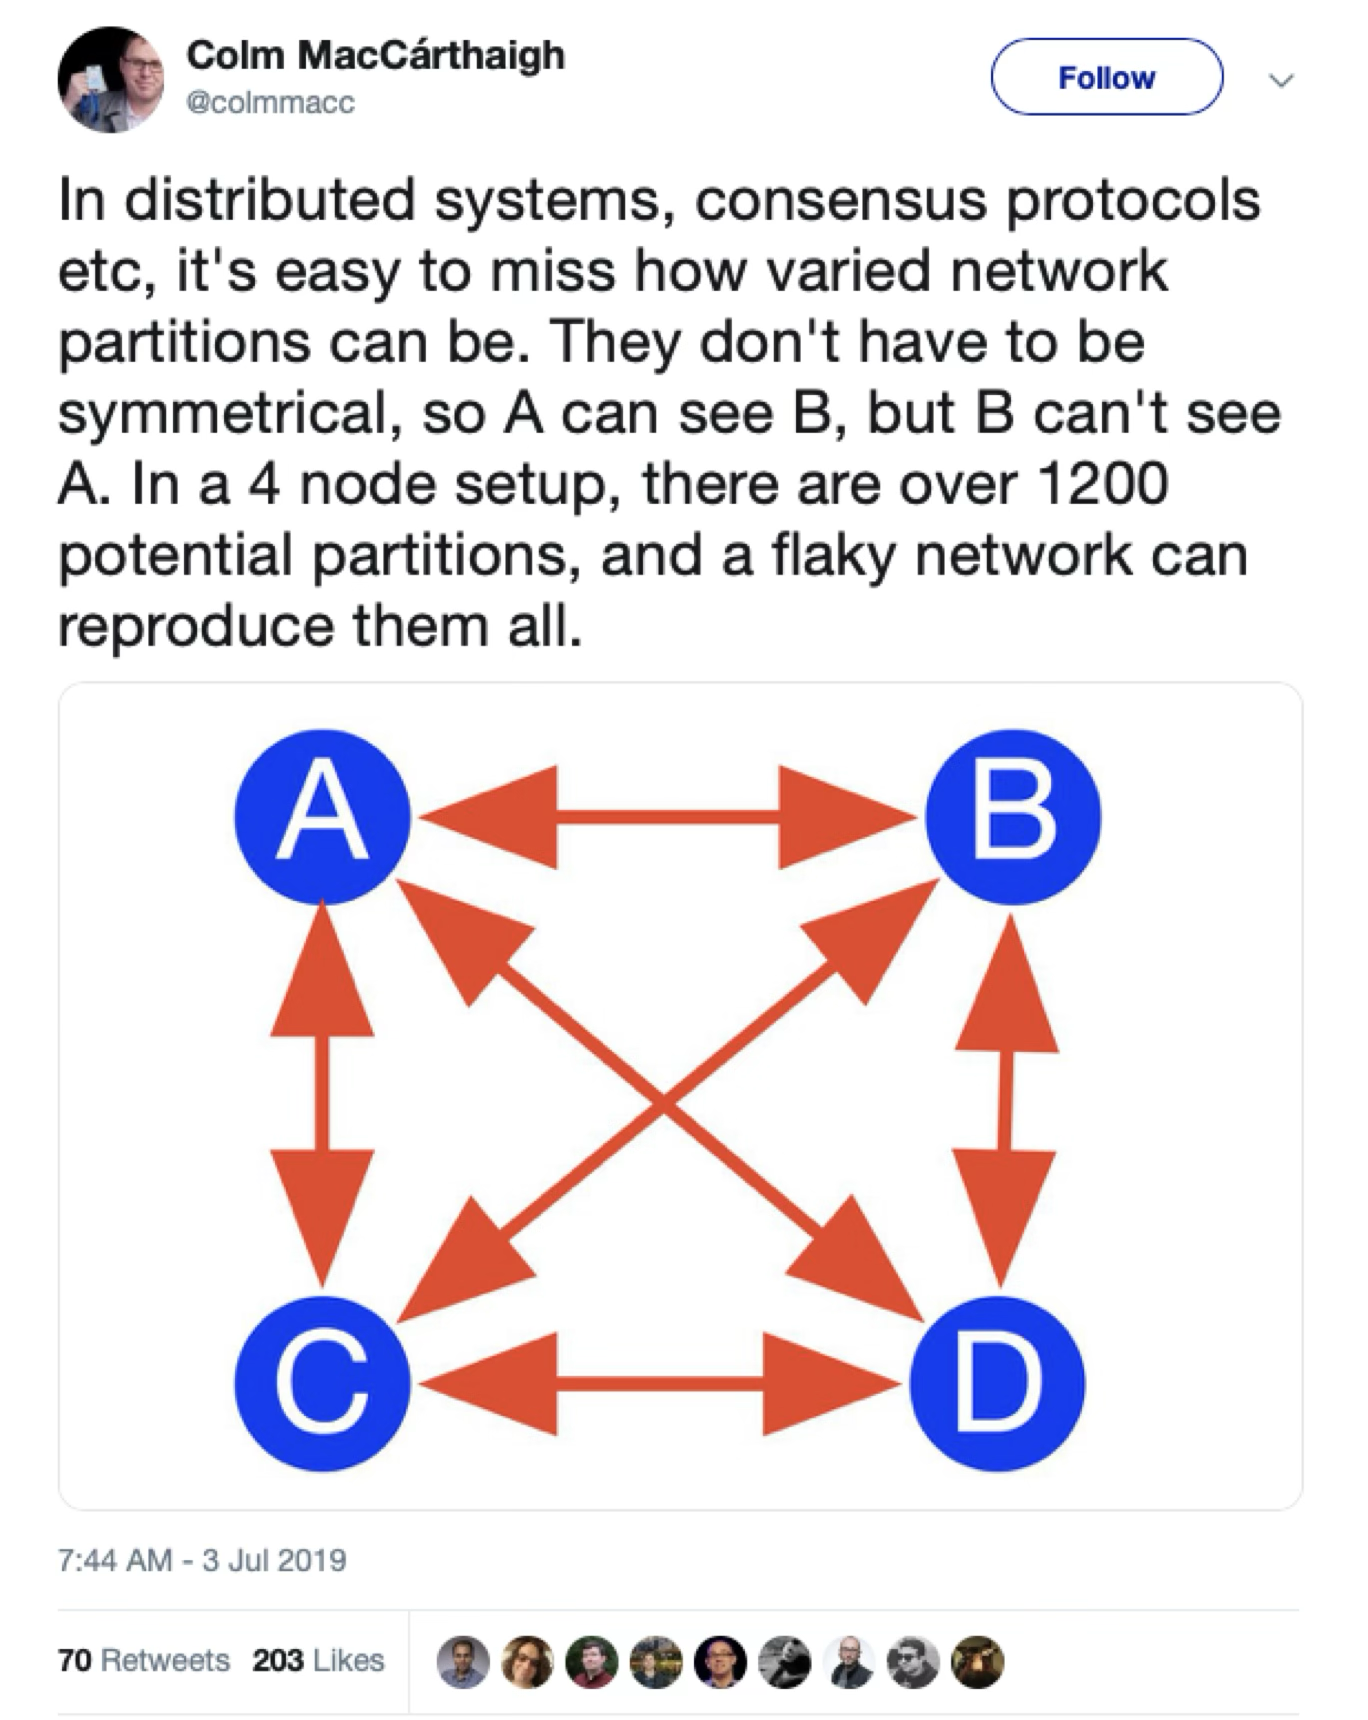
\includegraphics[width=\linewidth]{../figures/Flakey-Network.png}}
%  \caption{\href{https://x.com/colmmacc/status/1146429508993503234?s=61}{X/Twitter}}
\end{marginfigure}

%In distributed systems, consensus protocols etc, it's easy to miss how varied network partitions can be. They don't have to be symmetrical, so A can see B, but B can't see A. In a 4 node setup, there are over 1200 potential partitions, and a flakey network can reproduce them all.

Link failures are invisible (hidden) in a Clos. They are 100\% visible in an Æthernet 8-valency mesh: For 4 fully connected nodes, there are ($n(n-1)/2) = 6$ links. With 4 up/down unidirectional configurations on each link \{$\downarrow\downarrow ~~ \downarrow\uparrow ~~ \uparrow\downarrow ~~ \uparrow\uparrow$\}
% ${00, 01, 10, 11}$; 
 gives $4^6-1 = 4095$ possible failure modes. 
 
 \subsection{Where:}

%Depicted mathematically as \{$\downarrow\downarrow ~~ \downarrow\uparrow ~~ \uparrow\downarrow ~~ \uparrow\uparrow$\}

\begin{description}
	\item  [$\downarrow\downarrow$] Down from Alice's perspective, Down from Bob's perspective.
	\item  [$\downarrow\uparrow$] Down from Alice's perspective, Up from Bob's perspective.
	\item  [$\uparrow\downarrow$] Up from Alice's perspective, Down from Bob's perspective.
	\item  [$ \uparrow\uparrow$] Up from Alice's perspective, Up from Bob's perspective.
\end{description}

\marginnote{These are only the clean (binary) failures --  flakey connections are much worse! This makes conventional reliability calculations at least 1200 times worse than it looks from a simple series/parallel perspective -- for distributed systems}


\end{document}